\documentclass[12pt,letterpaper,noanswers]{exam}
\usepackage[usenames,dvipsnames,svgnames,table]{xcolor}
\usepackage[margin=0.9in]{geometry}
\renewcommand{\familydefault}{\sfdefault}
\usepackage{tikz}
\usepackage{multicol}
\pagestyle{head}
\header{AM 111 Class 23}{}{Artificial Neural Networks, p.\thepage}
\runningheadrule
\headrule
\usepackage{siunitx}
\usepackage{graphicx} % more modern
\usepackage{amsmath} 
\usepackage{amssymb} 
\usepackage{hyperref}
\usepackage{tcolorbox}
\usepackage{enumitem}
\def\mbf{\mathbf}
\newcommand{\vc}[1]{\boldsymbol{#1}}
\def\dsst{\displaystyle}
\DeclareMathOperator*{\argmin}{arg\,min} % thin space, limits underneath in displays
\usepackage{listings}
\newcommand{\note}[1]{{#1}} % show notes in red
%\renewcommand{\note}[1]{} % don't display notes

\begin{document}
 \pdfpageheight 11in 
  \pdfpagewidth 8.5in

\noindent 

\section*{Preliminaries}


\begin{itemize}
\itemsep0pt
\item The project log for this week is due on Monday Nov 27.
\item The skill check on Tuesday will be the final two retakes.
\end{itemize}


\noindent\textbf{Big picture}

Today: modeling nonlinear functions using artificial neural networks

\vspace{0.2cm}
\hrule
\vspace{0.2cm}

\noindent \textbf{Skill check practice}

No new skill


\vspace{0.2cm}
\hrule
\vspace{0.2cm}


\section*{A tiny bit of machine learning}
\note{The term \emph{machine learning} can refer to many methods, from statistical methods (including principle component analysis), to techniques used to create assistive driving algorithms.

A common problem is one of \textbf{classification}.  An input belongs to a category: given an input, $\vc{x}$, identify its category, $y$.

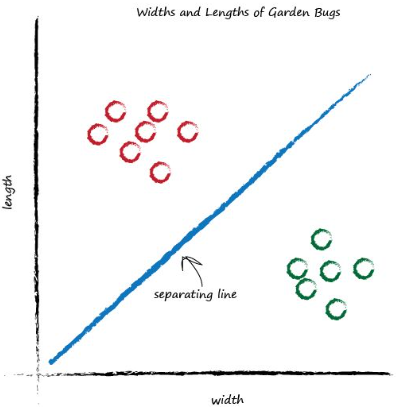
\includegraphics[scale=0.4]{img/C22rashidbugs.png}
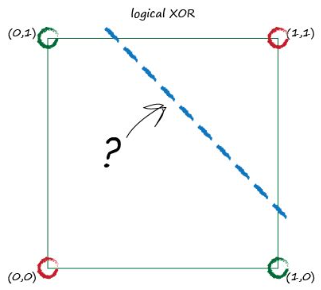
\includegraphics[width=0.4\linewidth]{img/C22rashidxor1.png}

Figures from Rashid 2016 \cite{rashid2016make}

In the example on the left a line is being used to classify two kinds of bugs.

In the example on the right, a single line fails as a classifier.}

\subsection*{Artificial neural nets (ANN)}

(definitions from  Goodfellow et al \S 6 \cite{Goodfellow-et-al-2016})
\note{
\begin{tcolorbox}

\begin{itemize}
\itemsep0pt
    \item A classifier, $f^*$, takes an input $\vc{x}$ and maps it to a category, $y$: $y = f^*(\vc{x})$.
    \item A \textbf{feedforward neural network} defines a mapping $\vc{y} = f(\vc{x};\vc{\theta})$, where the parameters $\vc{\theta}$ are \textbf{learned} to create an approximation of $f^*$. 
\end{itemize}
\end{tcolorbox}}

\renewcommand{\inputnum}{4} 
% Hidden layer neurons'number
\renewcommand{\hiddennum}{5} 
% Hidden layer neurons'number
\renewcommand{\hiddennumk}{4}  
% Output layer neurons'number
\renewcommand{\outputnum}{2} 
\begin{tikzpicture}
% Input Layer
\foreach \i in {1,...,\inputnum}
{
    \node[circle, 
        minimum size = 6mm,
        fill=orange!30] (Input-\i) at (0,-\i) {};
}
% Hidden Layer
\foreach \i in {1,...,\hiddennum}
{
    \node[circle, 
        minimum size = 6mm,
        fill=teal!50,
        yshift=(\hiddennum-\inputnum)*5 mm
    ] (Hidden-\i) at (2.5,-\i) {};
}
\foreach \i in {1,...,\hiddennumk}
{
    \node[circle, 
        minimum size = 6mm,
        fill=teal!50,
        yshift=(\hiddennumk-\inputnum)*5 mm
    ] (Hiddenk-\i) at (5,-\i) {};
}
% Output Layer
\foreach \i in {1,...,\outputnum}
{
    \node[circle, 
        minimum size = 6mm,
        fill=purple!50,
        yshift=(\outputnum-\inputnum)*5 mm
    ] (Output-\i) at (7.5,-\i) {};
}
% Connect neurons In-Hidden
\foreach \i in {1,...,\inputnum}
{
    \foreach \j in {1,...,\hiddennum}
    {
        \draw[->, shorten >=1pt] (Input-\i) -- (Hidden-\j);   
    }
}
% Connect neurons Hidden-Out
\foreach \i in {1,...,\hiddennum}
{
    \foreach \j in {1,...,\hiddennumk}
    {
        \draw[->, shorten >=1pt] (Hidden-\i) -- (Hiddenk-\j);
    }
}
\foreach \i in {1,...,\hiddennumk}
{
    \foreach \j in {1,...,\outputnum}
    {
        \draw[->, shorten >=1pt] (Hiddenk-\i) -- (Output-\j);
    }
}
% Inputs
\foreach \i in {1,...,\inputnum}
{     
    \draw (Input-\i) node {$x_{\i}$};
    % \draw[<-, shorten <=1pt] (Input-\i) -- ++(-0.5,0)
    %     node[left]{$x_{\i}$};
}
% Outputs
\foreach \i in {1,...,\outputnum}
{            
\draw (Output-\i) node {$y_{\i}$};
    % \draw[->, shorten <=1pt] (Output-\i) -- ++(0.5,0)
    %     node[right]{$y_{\i}$};
}
\end{tikzpicture}
\note{
\begin{tcolorbox}
\begin{itemize}
\itemsep0pt
    \item The term \textbf{network} is used because different functions are composed together according to the connections in a directed graph.  For a feedforward model the graph is acyclic.  
    \item $f(\vc{x}) = f^{(k)}(...(f^{(2)}(f^{(1)}(\vc{x}))))$ where $f^{(1)}$ is the \textbf{first layer} of the network, $f^{(2)}$ the \textbf{second layer}, etc.  The final layer is the \textbf{output layer}.
    \item The length of the chain of composed functions is the \textbf{depth} of the model.
    \item The output layer should produce a value close to $y$.  The output of other layers is not specified by the model: these are the \textbf{hidden layers}.
\end{itemize}
\end{tcolorbox}
}
\begin{enumerate}[resume=classQ]
\item For the network at the top of the page:
\begin{parts}
\item What is its depth?
\item How many hidden layers does it have?
\item A layer consists of \textbf{units} (also called \textbf{nodes}).  How many units are in the hidden layers?
\vspace{1cm}
\end{parts}
\end{enumerate}
\note{
\begin{tcolorbox}
\begin{itemize}
\itemsep0pt
    \item A model is called \textbf{feedforward} when there are no feedback connections via which outputs of the model are fed back into the model.
    
    \item The term \textbf{neural} is used because aspects of the modeling are inspired by ideas from neuroscience.
\end{itemize}
\end{tcolorbox}
}
% tikz code from https://latexdraw.com/drawing-neural-networks-in-tikz-short-guide/
% Input layer neurons'number
\renewcommand{\inputnum}{2} 
% Hidden layer neurons'number
\renewcommand{\hiddennum}{2}  
% Output layer neurons'number
\renewcommand{\outputnum}{1} 
 
\hfill
\begin{tikzpicture}
 
% Input Layer
\foreach \i in {1,...,\inputnum}
{
    \node[circle, 
        minimum size = 6mm,
        fill=orange!30] (Input-\i) at (0,-\i) {};
}
 
% Hidden Layer
\foreach \i in {1,...,\hiddennum}
{
    \node[circle, 
        minimum size = 6mm,
        fill=teal!50,
        yshift=(\hiddennum-\inputnum)*5 mm
    ] (Hidden-\i) at (2.5,-\i) {};
}
 
% Output Layer
\foreach \i in {1,...,\outputnum}
{
    \node[circle, 
        minimum size = 6mm,
        fill=purple!50,
        yshift=(\outputnum-\inputnum)*5 mm
    ] (Output-\i) at (5,-\i) {};
}
 
% Connect neurons In-Hidden
\foreach \i in {1,...,\inputnum}
{
    \foreach \j in {1,...,\hiddennum}
    {
        \draw[->, shorten >=1pt] (Input-\i) -- (Hidden-\j);   
    }
}
 
% Connect neurons Hidden-Out
\foreach \i in {1,...,\hiddennum}
{
    \foreach \j in {1,...,\outputnum}
    {
        \draw[->, shorten >=1pt] (Hidden-\i) -- (Output-\j);
    }
}
 
% Inputs
\foreach \i in {1,...,\inputnum}
{
\draw (Input-\i) node {$x_{\i}$};
    % \draw[<-, shorten <=1pt] (Input-\i) -- ++(-0.5,0)
    %     node[left]{$x_{\i}$};
}
 
% Outputs
\foreach \i in {1,...,\outputnum}
{          
\draw (Output-\i) node {$y_{\i}$};
    % \draw[->, shorten <=1pt] (Output-\i) -- ++(0.5,0)
    %     node[right]{$y_{\i}$};
}


\draw[-stealth] (Output-1) -- ++(0,1) -- ++(-3,0) -- (Hidden-1);

 
\end{tikzpicture}
\hfill
\begin{tikzpicture}
 
% Input Layer
\foreach \i in {1,...,\inputnum}
{
    \node[circle, 
        minimum size = 6mm,
        fill=orange!30] (Input-\i) at (0,-\i) {};
}
 
% Hidden Layer
\foreach \i in {1,...,\hiddennum}
{
    \node[circle, 
        minimum size = 6mm,
        fill=teal!50,
        yshift=(\hiddennum-\inputnum)*5 mm
    ] (Hidden-\i) at (2.5,-\i) {};
}
 
% Output Layer
\foreach \i in {1,...,\outputnum}
{
    \node[circle, 
        minimum size = 6mm,
        fill=purple!50,
        yshift=(\outputnum-\inputnum)*5 mm
    ] (Output-\i) at (5,-\i) {};
}
 
% Connect neurons In-Hidden
\foreach \i in {1,...,\inputnum}
{
    \foreach \j in {1,...,\hiddennum}
    {
        \draw[->, shorten >=1pt] (Input-\i) -- (Hidden-\j);   
    }
}
 
% Connect neurons Hidden-Out
\foreach \i in {1,...,\hiddennum}
{
    \foreach \j in {1,...,\outputnum}
    {
        \draw[->, shorten >=1pt] (Hidden-\i) -- (Output-\j);
    }
}
 
% Inputs
\foreach \i in {1,...,\inputnum}
{     
    \draw (Input-\i) node {$x_{\i}$};
    % \draw[<-, shorten <=1pt] (Input-\i) -- ++(-0.5,0)
    %     node[left]{$x_{\i}$};
}
 
% Outputs
\foreach \i in {1,...,\outputnum}
{            
\draw (Output-\i) node {$y_{\i}$};
    % \draw[->, shorten <=1pt] (Output-\i) -- ++(0.5,0)
    %     node[right]{$y_{\i}$};
}
\end{tikzpicture}
\hfill

\begin{enumerate}[resume=classQ]
\item The networks above have an input layer, $x_1$, $x_2$, a hidden layer, and an output layer, $y_1$.  Which network is feedforward?  \emph{The other is called `recurrent'}.
\vspace{1cm}

\end{enumerate}
%$y_1 = f^{(2)}(f^{(1)}(\vc{x}; \vc{\theta}))$

\note{
\begin{tcolorbox}
(notation from Koumoutsakos et al notes \S 9)

The \textbf{input} to node $j$ in layer $k$, $a_{j}^k$, is a weighted sum of the contributions from the nodes, $i$, in the previous layer, added to a constant term, called the \textbf{bias}. 

For unit $j$ in the first layer, \[a_j^1 = \sum\limits_{i=1}^{n_0} w_{ji}^1x_i + w_{j0}^1.\]

Extend the inputs with $x_0 = 1$, so $a_j^1 = \sum\limits_{i=0}^{n_0} w_{ji}^1x_i = W^1\vc{x}$ where $W^1$  is a matrix with elements $W^1_{ji} = w^1_{ji}$.

The \textbf{output} of the first layer $z_j^1 = \varphi_1(a_j^1)$ where $\varphi_1$ is the first layer \textbf{activation function}.
\end{tcolorbox}
}
\vspace{1in}

\renewcommand{\inputnum}{3} 
\renewcommand{\hiddennum}{3}
\begin{tikzpicture}
% Input Layer
\foreach \i in {1,...,\inputnum}
{
    \node[circle, 
        minimum size = 6mm,
        fill=orange!30] (Input-\i) at (0,-\i) {};
}
% Hidden Layer
\foreach \i in {1,...,\hiddennum}
{
    \node[circle, 
        minimum size = 6mm,
        fill=teal!50,
        yshift=0*5 mm
    ] (Hidden-\i) at (2.5,-\i) {};
}
% Output Layer
\foreach \i in {1,...,\outputnum}
{
    \node[circle, 
        minimum size = 6mm,
        fill=purple!50,
        yshift=(\outputnum-\inputnum)*5 mm
    ] (Output-\i) at (5,-\i) {};
}
% Connect neurons In-Hidden
\foreach \i in {1,...,\inputnum}
{
    \foreach \j in {2,...,\hiddennum}
    {
        \draw[->, shorten >=1pt] (Input-\i) -- (Hidden-\j);   
    }
}
% Connect neurons Hidden-Out
\foreach \i in {1,...,\hiddennum}
{
    \foreach \j in {1,...,\outputnum}
    {
        \draw[->, shorten >=1pt] (Hidden-\i) -- (Output-\j);
    }
}
% Inputs
\draw (Input-1) node {$1$};
\draw (Input-2) node {$x_1$};
\draw (Input-3) node {$x_2$};
\draw (Hidden-1) node {$1$};
\draw (Hidden-2) node {$z^1_1$};
\draw (Hidden-3) node {$z^1_2$};
% Outputs
\foreach \i in {1,...,\outputnum}
{            
\draw (Output-\i) node {$y_{\i}$};
    % \draw[->, shorten <=1pt] (Output-\i) -- ++(0.5,0)
    %     node[right]{$y_{\i}$};
}
\end{tikzpicture}
\begin{enumerate}[resume=classQ]
    \item For the neural network above, how many inputs does it have?  How many units in the hidden layer?  How many layers is the network? What is the purpose of the nodes labeled `1'?
    \vspace{1cm}
\end{enumerate}

\subsection*{Example: modeling XOR with a neural net (from Goodfellow et al \S 6.1)}

\note{
$f^*$ is given by the XOR function (limit ourselves to these inputs):

\begin{tabular}{c | c|| c}
$x_1$ & $x_2$ & $y_1$ \\
\hline
0 & 0 & 0 \\
0 & 1 & 1 \\
1 & 0 & 1 \\
1 & 1 & 0 
\end{tabular}


Choose one hidden layer, so this is a $2$-layer neural network.

\[f(\vc{x}; W^1, W^2) = \varphi_2(W^2\varphi_1(W^1\vc{x})),\] where $W^1, W^2$ are weight matrices, and the activation functions $\varphi_1$ and $\varphi_2$ act elementwise on their vector inputs.
}

Choose the activation function $\max\{0,a\}$ for $\varphi_1$.  Let $\varphi_2 = 1$

\begin{enumerate}[resume=classQ]
    \item Plot the activation function $\varphi(x) = \max\{0,x\}$ for the domain $-2<x<2$.  \emph{This function is called the rectified linear activation function.}
    \vspace{1in}
    \item Let $W^1 = \left[\begin{array}{r r r}
    0 & 1 & 1 \\
    -1 & 1 & 1 \\
    \end{array}\right]$, $W^2 = [\begin{array}{r r r}
    0 & 1 & -2
    \end{array}]$.  There are four sets of inputs $(1, x_1, x_2)$.
    \begin{parts}
    \item (Worked as an example) 
    
    Set $x_1 = 0$ and $x_2 = 0$.  So $\vc{x} = \left[\begin{array}{r}
    1 \\ 0 \\ 0
    \end{array}\right]$.  The model gives: 
    
    (1) $W^1\vc{x} = \left[\begin{array}{r}0 \\ -1\end{array}\right]$.
    
    (2) $\varphi_1(W^1\vc{x}) = \max\{0,\left[\begin{array}{r}0 \\ -1\end{array}\right]\} = \left[\begin{array}{r}0 \\ 0\end{array}\right]$.  Then augment this with $z_0$ to get $\left[\begin{array}{r}1 \\ 0 \\ 0\end{array}\right]$
    
    (3) $W^2\varphi_1(W^1\vc{x}) = W^2 \left[\begin{array}{r}1 \\0 \\ 0\end{array}\right] = 0$
    
    (4) $\varphi_2(W^2\varphi_1(W^1\vc{x})) = W^2\varphi_1(W^1\vc{x}) = 0$
    
    This matches the expected value of $y_1$.
    
    \item Set $x_1 = 1$ and $x_2 = 1$.  Check whether the output of the model matches the expected value of $y_1$ from the table.
    \vspace{1.5in}
    \end{parts}
\end{enumerate}
\note{
\noindent  Set $X = \left[\begin{array}{r r r r} 1 & 1 & 1 & 1 \\
0 & 0 & 1 & 1 \\
0 & 1 & 0 & 1\end{array}\right]$.  $W^1X = \left[\begin{array}{r r r r}
0 & 1 & 1 & 2 \\
-1 & 0 & 0 & 1\end{array}\right]$

\noindent  These are the $a_j^1$, and they lie along a line with slope $1$ in $2$-space.

\noindent  Applying the nonlinear activation function:
$\varphi_1(W^1X) = \left[\begin{array}{r r r r}
0 & 1 & 1 & 2 \\
0 & 0 & 0 & 1\end{array}\right]$.  These are the $z_j^1$ and the are no longer on a line.

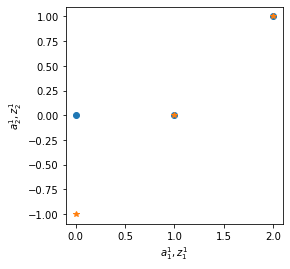
\includegraphics[scale=0.5]{img/C22az.png}

\noindent  Extending with $z_0^1$ we have $\left[\begin{array}{r r r r}
1 & 1 & 1 & 1\\
0 & 1 & 1 & 2 \\
0 & 0 & 0 & 1\end{array}\right]$.  $W^2\vc{z}^1 = \left[\begin{array}{r r r} 0 & 1 & -2\end{array}\right]\left[\begin{array}{r r r r}
1 & 1 & 1 & 1\\
0 & 1 & 1 & 2 \\
0 & 0 & 0 & 1\end{array}\right] = \left[\begin{array}{r r r r} 
0 & 1 & 1 & 0
\end{array}\right]$

\noindent  This neural network exactly captures the nonlinear XOR function.
}
\subsection*{Activation functions}

(See Koumoutsakos notes \S 9.3)
\note{
\begin{tcolorbox}
In the XOR example above we encountered two activation functions:
\begin{itemize}
\itemsep0pt
    \item \textbf{identity}: $\varphi(x) = x$
    \item \textbf{rectified linear unit} (ReLU): $\varphi(x) = \left\{\begin{array}{r r}
    0 & \text{if }x\leq 0 \\
    x & \text{if }x>0\end{array}\right.$
\end{itemize}
Smooth switching functions such as $\tanh x$ (\textbf{hyperbolic tangent}), or $\dfrac{1}{1+e^{-x}}$ (\textbf{logistic}) are also common.
\end{tcolorbox}
}
\begin{enumerate}[resume=classQ]
\item $\tanh x = \dfrac{\sinh x}{\cosh x}$ where $\sinh x = \frac{1}{2}\left(e^{x}-e^{-x}\right)$ and $\cosh x = \frac{1}{2}\left(e^{x}+e^{-x}\right)$, so $\tanh x = \dfrac{e^x-e^{-x}}{e^x+e^{-x}}$.

\begin{parts}
\item At $x = 0$, find $\dfrac{e^x-e^{-x}}{e^x+e^{-x}}$.
\item As $x\rightarrow\infty$, $e^{-x}$ approaches $0$.  What does $\tanh x$ approach in this limit?
\vspace{1cm}
\item As $x\rightarrow -\infty$, $e^{x}$ approaches $0$.  What does $\tanh x$ approach in this limit?
\vspace{1cm}
\item Near $0$, $e^x \approx 1 + x$ and $e^x\approx 1-x$.  Combine these Taylor expansions to create an approximation for $\tanh x$ near $0$.
\vspace{1cm}
\end{parts}

Sketch an approximate plot of $\tanh x$ using the information you've found above.  Do \textbf{not} use a calculator or other plotting software.
\vspace{1.5in}

\item Provide similar information for the logistic function.

Near $x=0$:

$(1+e^{-x})^{-1}\approx (2-x)^{-1} = \dfrac{1}{2}(1-x/2)^{-1} \approx \dfrac{1}{2}(1+x/2)$
\end{enumerate}
\vspace{1.7in}

\subsection*{Training}
\note{In the XOR example, the weights were given.  In general, the weights need to be determined for each layer of the neural net.
\begin{tcolorbox}
Train on data $d_n = \{\vc{x}_n,\hat{\vc{y}}_n\}$ where $n=1,...,N$.  Find weights $\vc{w} = \{W^1,W^2,...,W^L\}$ to minimize the error between the observations and the model output.

For now we will consider the $2$-norm for the error function.  See \cite{Goodfellow-et-al-2016} \S 6.2.2.2 and \S 6.2.2.3 for a discussion of other choices of error function for particular problem types.
\end{tcolorbox}
}


\subsection*{Finding the weights: gradient descent}

\note{
In our neural network example from the previous class, the weight matrices were taken as given.

In general, weights need to be determined for each layer of the neural net.
\begin{tcolorbox}
Given \textbf{training} data $d_n = \{\vc{x}_n,\hat{\vc{y}}_n\}$ where $n=1,...,N$.  Find weights $\vc{w} = \{W^1,W^2,...,W^L\}$ to minimize the \textbf{error} between the observations, $\hat{\vc{y}}_n$ and the model output.

This is an optimization problem.

%For now we will consider the $2$-norm for the error function.  See \cite{Goodfellow-et-al-2016} \S 6.2.2.2 and \S 6.2.2.3 for a discussion of other choices of error function for particular problem types.
\end{tcolorbox}

With an $L$ layer feedforward neural network, our model is \[\vc{y}(\vc{x}_n,\vc{w}) = \phi_L(W^L\phi_{L-1}(...\phi_2(W^2\phi_1(W^1\vc{x}))...)).\] This is a nonlinear function of $\vc{x}$, parameterized by $\vc{w}$.

The choice of error function should depend on the problem type.  See \cite{Goodfellow-et-al-2016} \S 6.2.2.2 and \S 6.2.2.3 for a discussion of choices of error function for categorical data.  For these notes, we will choose a sum of squares error.  Let \[E_n(\vc{w}) = \dfrac{1}{2}\left(\hat{\vc{y}}_n-\vc{y}(\vc{x}_n,\vc{w})\right)\cdot\left(\hat{\vc{y}}_n-\vc{y}(\vc{x}_n,\vc{w})\right).\]
Let the overall error on the training data set be the sum of the errors on individual input-output pairs.
\[E(\vc{w}) = \sum\limits_{n=1}^N E_n(\vc{w}).\]

The optimization problem is to find the set of weights, $\vc{w}^*$, that minimize $E$.  Nonlinearity of $\vc{y}$, and therefore of $E(\vc{w})$ means that optimization methods for finding a global optimum are unlikely to apply. Instead, use an iterative algorithm to improve the weights at each step $\vc{w}$ with a low error using an iterative, gradient based method.  

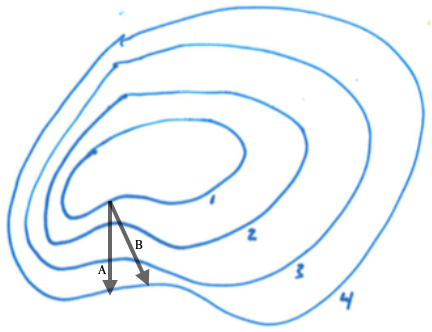
\includegraphics[scale=0.5]{img/C23gradient.png}
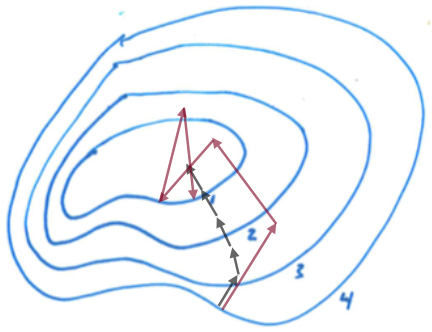
\includegraphics[scale=0.5]{img/C23gradientpath.png}
}
\begin{enumerate}[resume=classQ]
    \item The contour plots above are showing $E(w_1,w_2)$, a function of two weights.  Each labeled curve is a curve on which the function has a constant value ($E(w_1,w_2) = 3$, for example).
   
   In the plot on the left, one vector is labeled A and the other is labeled B.  Consider the vectors to be originating on the $E = 1$ contour.  Which vector is pointing in a direction closer to the gradient direction?
    \vspace{1cm}
   
\end{enumerate}
\note{
\begin{tcolorbox}
This algorithm is sometimes referred to as \textbf{stochastic gradient descent} (but it is not the only algorithm referred to with that terminology).
\begin{itemize}
\itemsep0pt
    \item Let $\vc{w}_1$ be a randomly generated initial set of weights.
    \item Choose one input-output pair from the training data, say $n$, and use the feedforward neural network model to generate $\vc{y}(\vc{x}_n,\vc{w}_1)$ and $E_ n(\vc{w}_1)$.
\item The gradient vector, $\nabla_{\vc{w}}E_n(\vc{w}_1)$ is a vector in the direction of fastest increase of $E_n$ at the point $\vc{w}_1$ (in the weight space). 
\item Update the weights: $\vc{w}_{k+1} = \vc{w}_k - \eta\nabla_{\vc{w}}E_n(\vc{w}_1)$.  $\eta$ is a scaling factor adjust the length of the gradient vector.  It is referred to as the \textbf{learning rate}.
\end{itemize}
\end{tcolorbox}
}


\begin{enumerate}[resume=classQ]
 \item In the plot on the right, each vector is drawn to be pointing in the direction of the negative of the gradient (where the gradient is calculated at the tail of the vector).  Which vector path was constructed using a higher learning rate?  How does the error evolve along on each of the paths?
\end{enumerate}

%\eject
% \noindent Below left: the number of connections between neurons in 10 examples of artificial neural networks, plotted vs the year they were published.

% \noindent Below right: the size of artificial neural networks for 20 examples, plotted vs the year they were published.

% 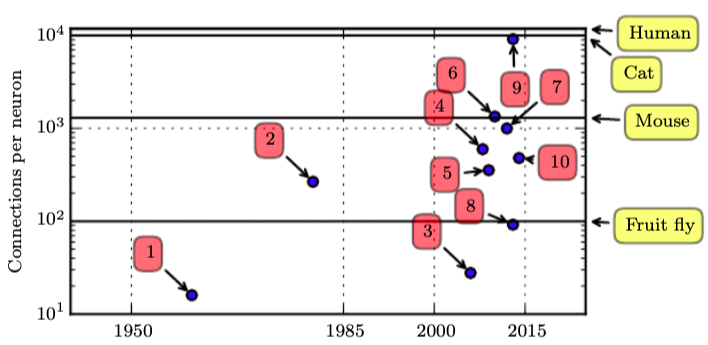
\includegraphics[width=0.45\linewidth]{img/C22neuronconnections.png}
% 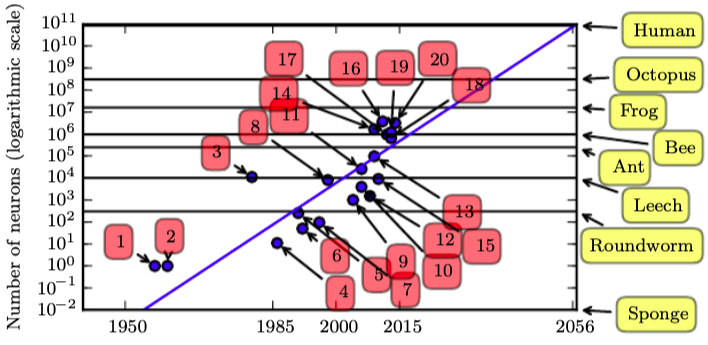
\includegraphics[width=0.45\linewidth]{img/C22neurons.png}
% \cite{Goodfellow-et-al-2016}
\vfill

\bibliographystyle{plain}
\bibliography{AM111references}
\end{document}